\documentclass[10pt,twocolumn,letterpaper]{article}

\usepackage{cvpr}
\usepackage{times}
\usepackage{epsfig}
\usepackage{graphicx}
\usepackage{amsmath}
\usepackage{amssymb}
\usepackage{graphicx}
\usepackage{subfig}
\usepackage{url}
\usepackage{varwidth}
\usepackage{multicol}
\usepackage{framed}

\usepackage[breaklinks=true,bookmarks=false]{hyperref}

\cvprfinalcopy
\begin{document}

%%%%%%%%% TITLE
\title{Friendly Streets: A Street View Classifier for Cautious Cyclists}

\author{Josh Sennett\\
University of Massachusetts, Amherst\\
{\tt\small jsennett@umass.edu}
\and
Evan Rourke\\
University of Massachusetts, Amherst\\
{\tt\small erourke@umass.edu}
}

\maketitle

%%%%%%%%% ABSTRACT
\begin{abstract}
The goal of this project is to classify street-view images as ``bike-designated'' or ``not''. Existing research has shown that convolutional neural networks (CNNs) are well-suited for scene classification and object detection, but have not been applied to classify bike-designation. The three contributions of this work are 1) to create a tool to generate high-quality datasets of street-view images labeled as bike-designated or not; 2) to develop a neural network to predict this label; and, 3) to establish a human baseline with which to compare the accuracy of our neural network. By fine-tuning a pre-trained ResNet neural network, we achieve 68.0\% overall accuracy on a test set of 3,454 unseen images, outperforming a human benchmark of 59.5\% on 1,313 images.
\end{abstract}

%%%%%%%%% INTRODUCTION
\section{Introduction}
\label{sec:intro}

Cyclists depend on routing applications to find safe and enjoyable bike routes. In these applications, roads may be ``bike-designated'' based on data from public records, privately-owned data sources, or open-source communities. The classification of bike-designation is often outdated, inaccurate, or unavailable, presenting a challenge for mapping software and cyclists to plan safe and optimal routes.

To approach this problem, we develop a convolutional neural network to classify street-view images of roads as bike-designated or not. We train our network on a dataset of street-view images labeled ``bike-designated'' or ``not'', which we generated by integrating OpenStreetMap \cite{osm} road classifications with Google's Street View API \cite{googlesv}.

``Bike-designation'' refers to whether a road contains infrastructure to make a road safer or more enjoyable for cyclists. OpenStreetMap, which we use as our source of road classification data, defines bike-designation as whether a roadway (for motor-vehicles) contains either a bike lane (a lane within a roadway) or a bike path (a lane alongside a roadway, but separated by a barrier). Bike-designated roads may also have shared-road arrows (``sharrows''), colored bike lanes, physical barriers, and cautionary (``share the road'') street signs.

\begin{figure}[t]
\begin{center}
	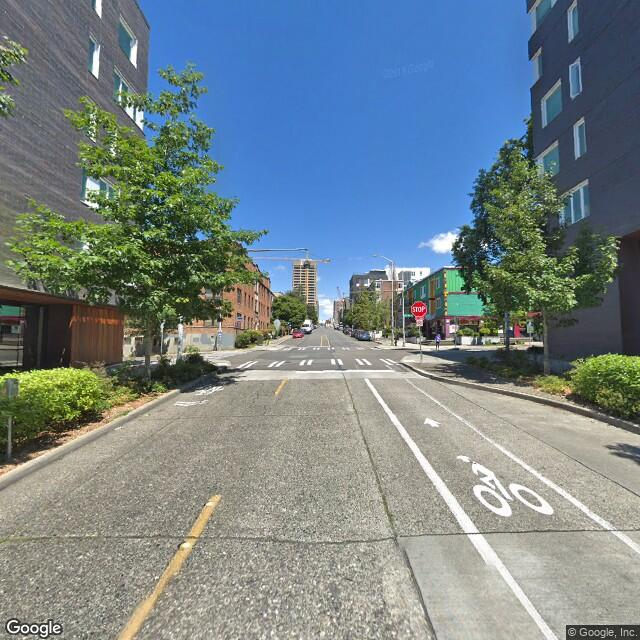
\includegraphics[width=0.4\linewidth]{intro1.jpg}
	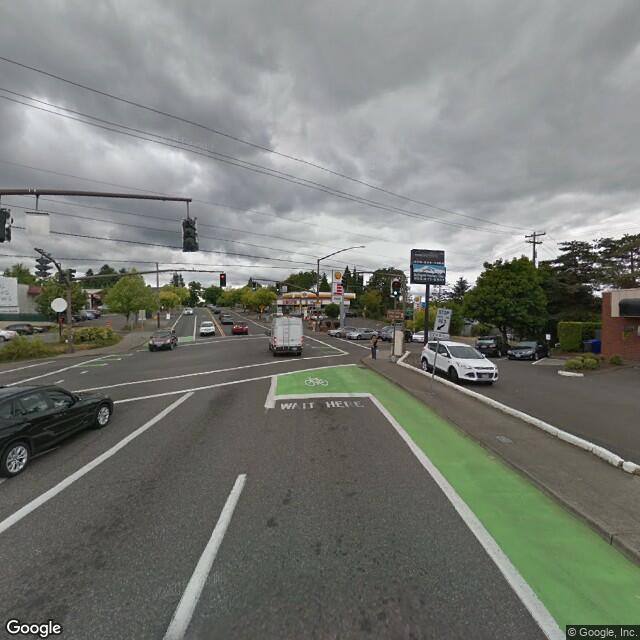
\includegraphics[width=0.4\linewidth]{intro7.jpg}
	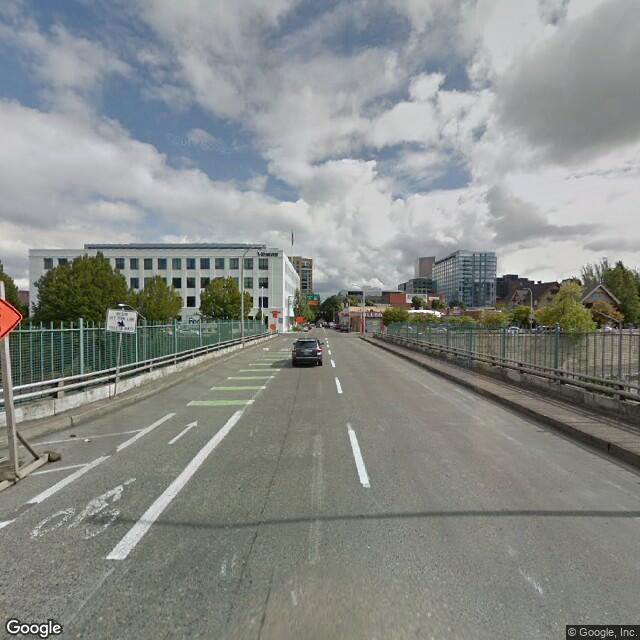
\includegraphics[width=0.4\linewidth]{intro4.jpg}
	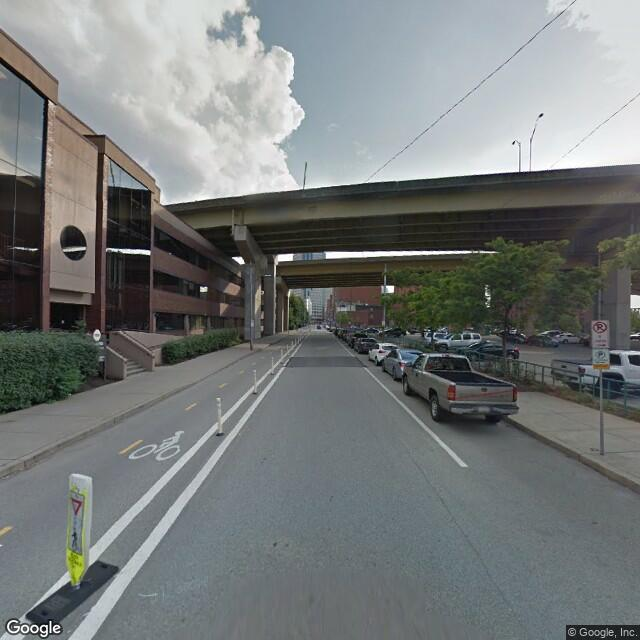
\includegraphics[width=0.4\linewidth]{intro5.jpg}
\end{center}
   \caption{Shared road markings (``sharrows''), colored bike lanes, and barriers are common features of bike-designated roads.}
\label{fig:long}
\label{fig:onecol}
\end{figure}


\begin{figure*}
  \centering
  \subfloat[Bike-designated]{
  	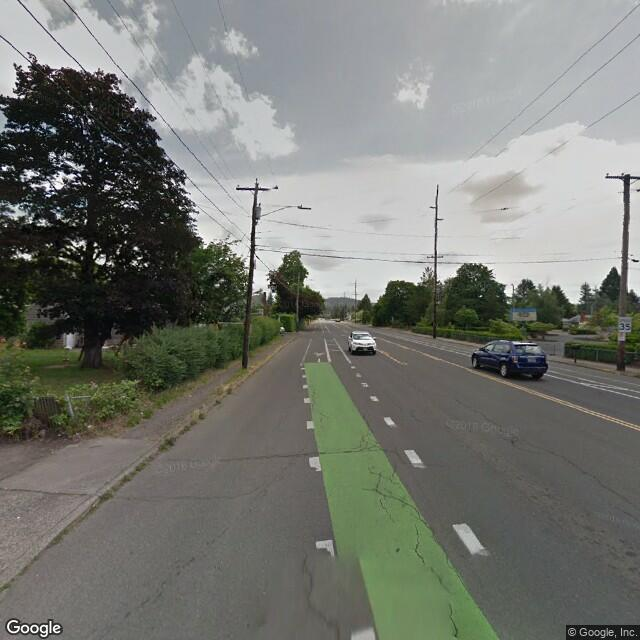
\includegraphics[width=0.1\textwidth]{intro2.jpg}\label{fig:f1}
  	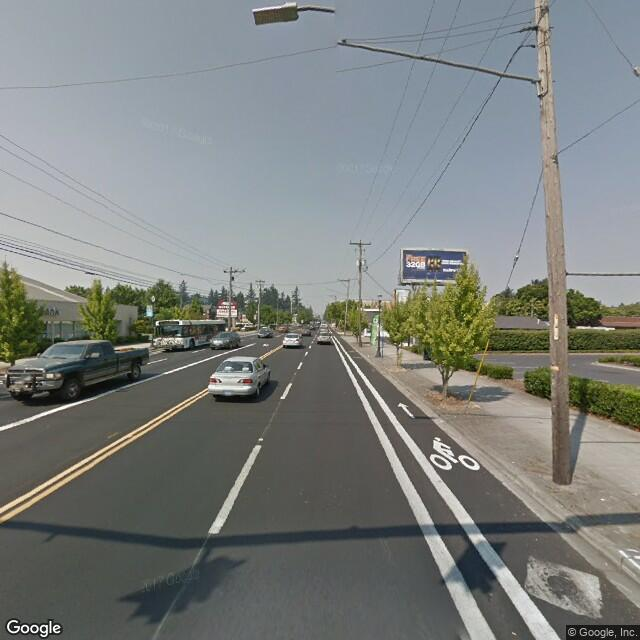
\includegraphics[width=0.1\textwidth]{intro3.jpg}\label{fig:f1}
  	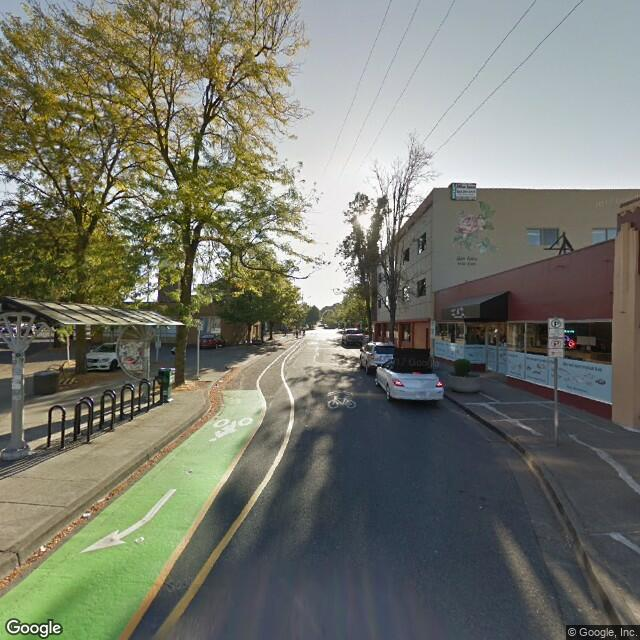
\includegraphics[width=0.1\textwidth]{intro6.jpg}\label{fig:f1}
  	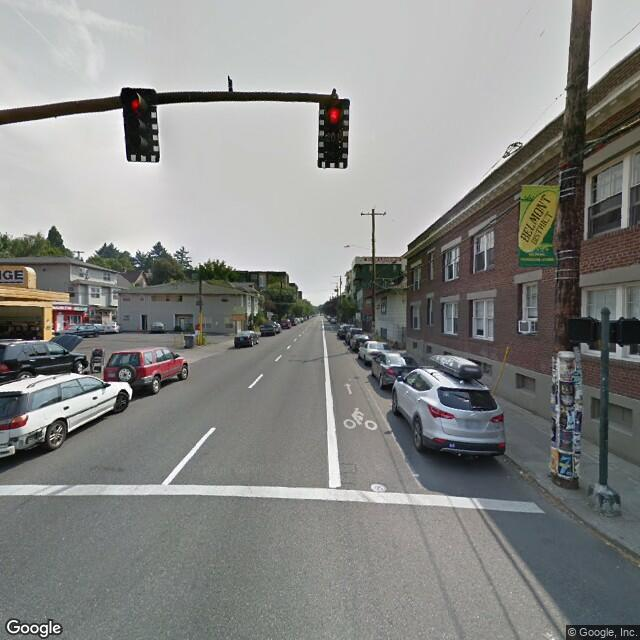
\includegraphics[width=0.1\textwidth]{intro8.jpg}\label{fig:f1}
	}
  \hfill
  \subfloat[Not bike-designated]{
  	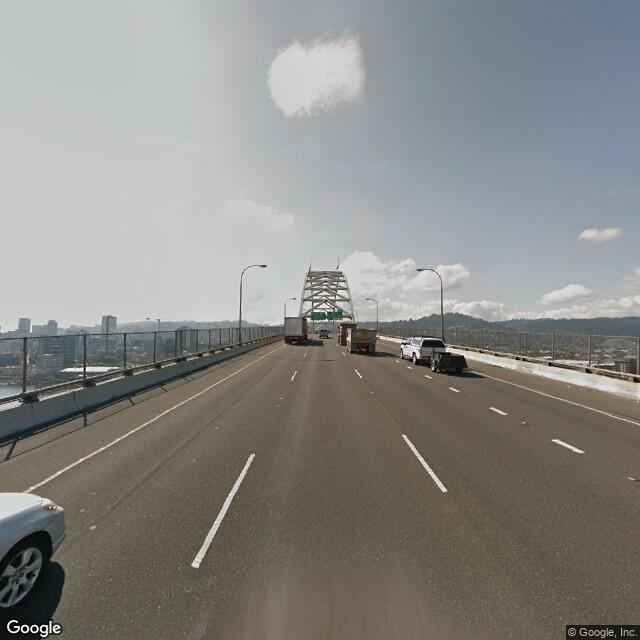
\includegraphics[width=0.1\textwidth]{intro9.jpeg}\label{fig:f1}
  	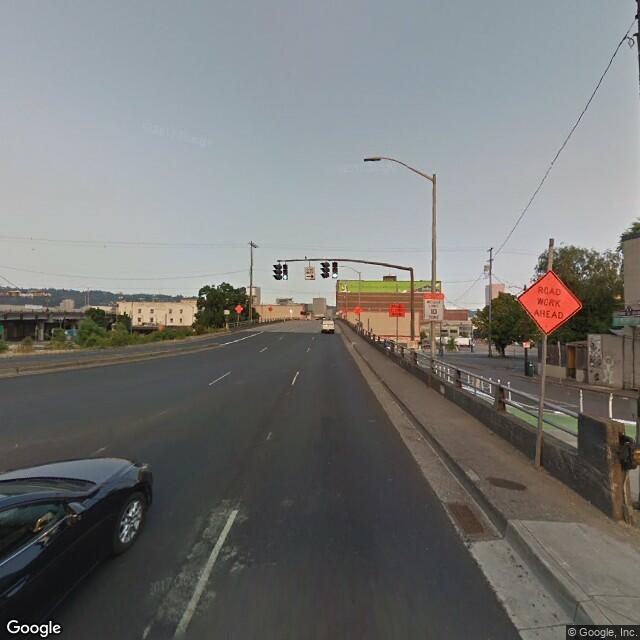
\includegraphics[width=0.1\textwidth]{intro10.jpg}\label{fig:f1}s
  	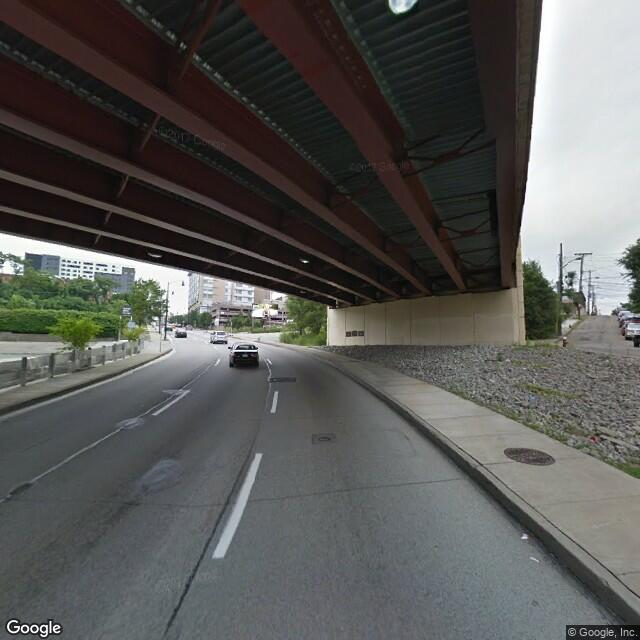
\includegraphics[width=0.1\textwidth]{intro11.jpg}\label{fig:f1}
  	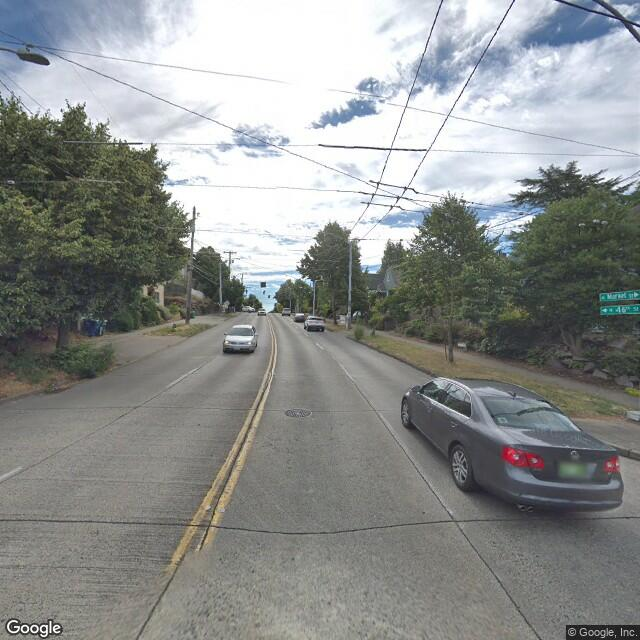
\includegraphics[width=0.1\textwidth]{intro12.jpeg}\label{fig:f1}
  }
  \caption{Example street-view images of bike-designated and not bike-designated roads.}
\end{figure*}

Developing a bike-designation street-view image classifier faces several challenges. First, there is no existing public, large-scale database of street-view images with the bike-designation label. Second, bike-designated roads contain a variety of different types of cycling infrastructure, and each type of infrastructure may look different depending on which city and country the road pertains to. Third, street-view images may not be positioned or oriented correctly to capture the relevant features. Last, street-view images are taken in real-world settings, and face several factors that decrease image quality including feature occlusion, background clutter, differences in illumination, and blur.

To overcome the first challenge, we generate a labeled dataset of street-view images by integrating OpenStreetMap road classification data with Google's Street View API. To overcome the remaining challenges, we develop a convolutional neural network to classify street-view images as bike-designated or not. Previous research has demonstrated the effectiveness of CNNs for scene understanding and object detection in real-world settings, where viewpoint variation, occlusion, background clutter, illumination, and intra-class variation are expected. 

The paper is structured as follows. Section \ref{sec:background} presents related research. Section \ref{sec:approach} explains our approach to developing a labeled dataset, neural network, and human baseline. Section \ref{sec:experiments} contains the results of our experiments to improve our network's performance. Section \ref{sec:conclusion} concludes with lessons learned and directions for future research.

%%%%%%%%% RELATED WORK
\section{Background and Related Work}
\label{sec:background}

\subsection{Scene Classification}
Convolutional neural networks have been widely successful in object classification tasks \cite{krizhevsky2012imagenet}. Trained on massive datasets, these networks have been able to nearly achieve or even exceed human performance benchmarks.

Scene classification, however, is a more challenging, generalized task than object classification: a scene class may be correlated with the presence of objects, but such objects may appear in other scene classes. Correctly classifying a scene depends not only on objects but also attributes (relating to spatial envelope, materials, lighting, and textures).

Xiao et al. developed the SUN Database, the first large-scale scene understanding database with 899 scene categories and over 130,000 labeled images \cite{xiao2010sun}. Shortly thereafter, Patterson and Hays developed the first large-scale scene attributes dataset and demonstrate the predictive power of attributes for classifying scenes \cite{6247998}. Most recently, Zhou et al. develop the Places database, a database of 434 scene categories and over 10 million scene images \cite{DBLP:journals/corr/ZhouKLTO16}. Using the Places database, Zhou et al. surpassed previous scene classification benchmarks using VGG, GoogLeNet, AlexNet, and ResNet convolutional neural networks. 

\subsection{Street View Images}
Several researchers have used Google Street View images as a source of natural images; Google Street View cars take panoramic photos along roads, providing a rich source of images of outdoor scenes. Netzer et al use Street View images to generate the Street View House Number dataset for digit classification. Similarly, Slavkovikj et al. use Street View images to develop a road-texture dataset for classification \cite{slavkovikj2014image}. Gebru et al. develop a car model classifier \cite{DBLP:journals/corr/GebruKWCDLF17}, and Hershey and Wulfe use deep learning to recognize geo-location from city Street View images \cite{hersheyrecognizing}.

%%%%%%%%% APPROACH
\section{Approach}
\label{sec:approach}

\subsection{Data}
To generate a labeled dataset of bike-designated street-view images, we created a tool to integrate OpenStreetMap road classifications with Google's Street View API. This tool does the following:
\begin{enumerate}
\item Download OpenStreetMap data for a particular region
\item Extract road segments (way elements) for this region using particular criteria
\item Extract road points (node elements) for these ways using particular criteria
\item Calculate road orientation for each for these nodes
\item Query Google's Street View API using node coordinates and road orientation
\item Save the street-view image with the road classifications
\end{enumerate}
Specifically, to create a dataset of bike-designated images, we did the following:

In step 1, we used OpenStreetMap data for four cities: Boulder, Pittsburgh, Portland, and Seattle. We chose these regions because of the quality and availability of bike-designation for roads in these cities, and because these cities have near-balance between bike-designated and non-designated roads (in total, 57\% and 43\%).

In step 2, we filtered road segments to only include road types ``motorway'', ``primary highway'', ``secondary highway'', and ``tertiary highway''. Other segment types included non-road segments not relevant to our analysis such as footpaths and bike-paths, as well as residential roads, which were often unlabeled with road classifications.

In step 3, we filtered nodes to only include the midpoint of each road. Given the cost of the Google Street View API (\$7 per 1000 images), we could not capture Street View images at all millions of nodes of all relevant highways. Nodes are typically several meters apart; so, capturing Street View images at adjacent nodes will result in similar images with a slightly shifted camera perspective. Extracting a single image for each road segment (rather than extracting multiple images at a subset of road segments) increases image heterogeneity while keeping our API costs reasonable.

In step 4, we determine the required camera orientation such that each image is pointed in the direction of the road. To do so, we calculate the geodesic azimuth (angular distance from north) between a node and the subsequent node. For one-way roads, we orient the camera to face in the forward-direction of the road.

In step 5, we query the API to determine if a Street View image is available for the given coordinate in a radius of 10 meters. We found that reducing the search radius to 10 meters decreased the chance that images of nearby (but different) roads were not accidentally downloaded in the case that a road did not have street-view images. Then, if an image is available, we download a 640x640 image using the node coordinate and the calculated camera orientation.

Finally, we randomly split our data into training, validation, and test sets using a 60-20-20 split. For training images, we applied random rotation, jitter, and horizontal flips; we resized images to 256x256 and center crop; and, we normalized images. For validation and test sets, we only resize, center crop, and normalize images.

\subsection{Neural Network}
Given the success of CNN classifiers for scene classification, we approach classifying bike-designation of street-view images by using CNN models. Specifically, we use a residual neural network (ResNet) architecture, which has ``shortcut connections'' that skip one or more convolutional layers to make training of deeper networks more efficient \cite{DBLP:journals/corr/HeZRS15}.

The classification of bike-designation can be considered a fine-grained scene classification task. To take advantage of the knowledge developed by state-of-the-art scene classifiers, we employ transfer learning by fine-tuning a pre-trained network. The goal of transfer learning is to apply the knowledge gained by a similar problem. In the context of deep learning, this implies using the weights of a pre-trained network as the initial weights of a new network. 

Fine-tuning involves modifying a pre-trained model to tune it to solve a different problem. Using a ResNet18 model, this implies (optionally) modifying and (necessarily) re-training one or more of the final layers of the model. With a small input dataset it is common to fix the parameters of some number of initial layers both to improve the performance of the model and to increase efficiency, by reducing the number of parameters to train. For these two reasons, we approached fine-tuning a pre-trained network by fixing all weights except for the final fully-connected layer, and then replacing the final layer with custom layers.

Given the similarity of our classification problem with the general task of scene classification, we use networks pre-trained on the Places365 scene classification dataset \cite{zhou2017places}. ResNet models pre-trained on Places365 are particularly suitable to our classification task because the convolutional layers have already learned low level features such as edges, shapes, spatial envelope, materials, lighting, and textures that are important predictors of scene classification. We chose ResNet18, rather than deeper versions of ResNet, because ResNet18 is faster to train (due to having fewer layers) while achieving comparable accuracy \cite{zhou2017places}.

In Section \ref{sec:experiments}, we discuss the different types of custom layers that we trained to develop our final model, visualized in Figure \ref{fig:model}.

\begin{figure}[t]
\begin{center}
	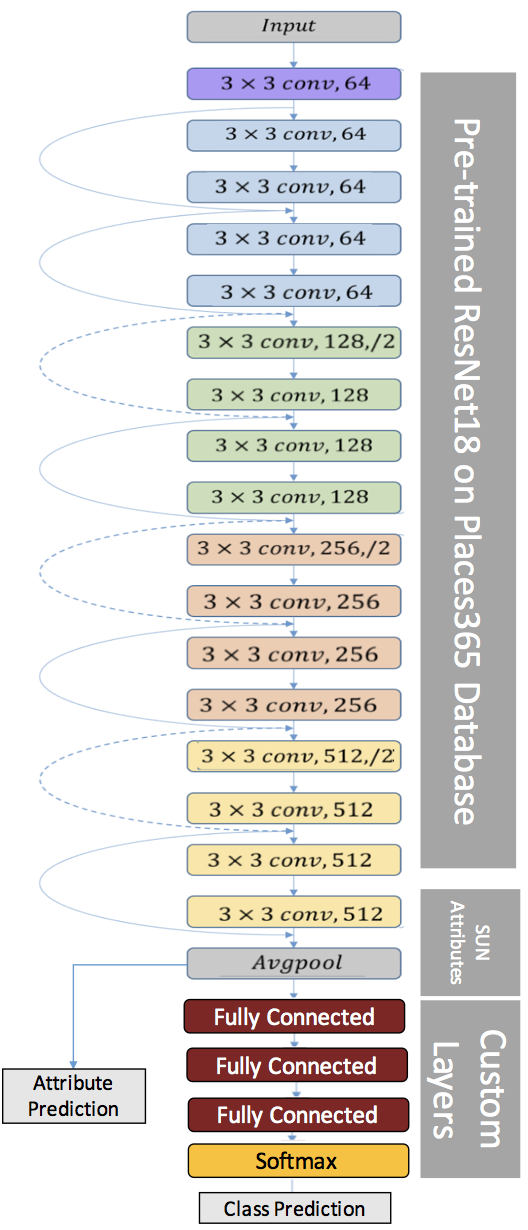
\includegraphics[width=.75\linewidth]{model.png}
\end{center}
	\caption{Final model: Pre-trained ResNet18 with three fine-tuned fully-connected layers.}
\label{fig:model}
\end{figure}

\subsection{Human Benchmark}
In order to evaluate our results, we developed a human benchmark with which to compare our network's classification accuracy. We created a cloud-hosted Jupyter Notebook to allow participants to predict the label of randomly selected images (Figure \ref{fig:ui}). Images were randomly selected from the full set of images. The user interface included a random image and two buttons that the user could press which submitted their prediction as ``not bike-designated'' or ``bike-designated''. Once pressed, a new randomly selected image would be loaded. Image accuracy was written to a private text file, hidden from the users; each user was shown their overall accuracy after they had completed labeling images. Section \ref{sec:quantitative} presents the results of the human benchmark, and compares it to the accuracy of our neural network.

\begin{figure}[t]
\begin{center}
	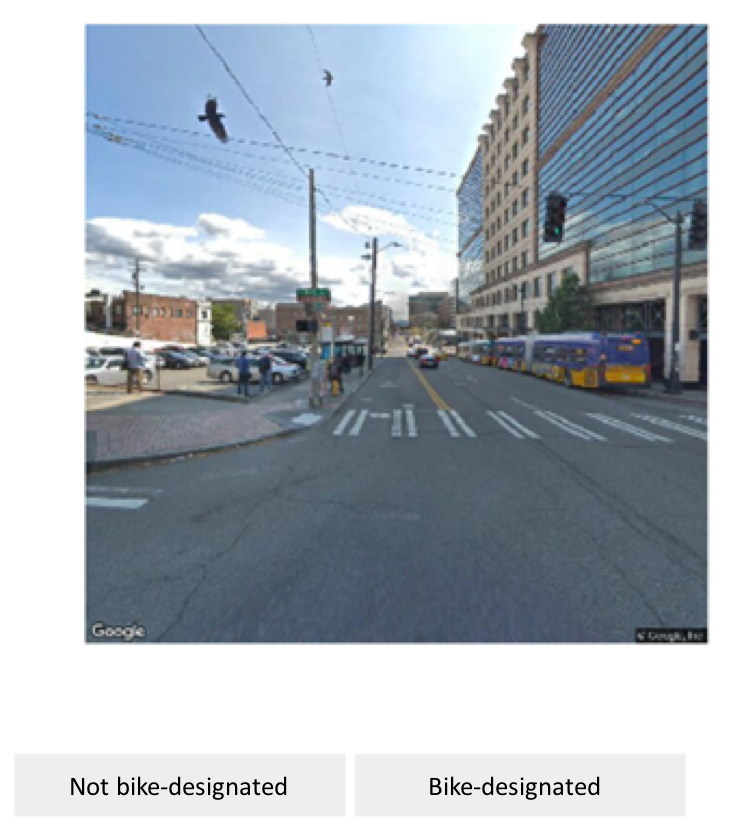
\includegraphics[width=.7\linewidth]{gui_2.png}
\end{center}
	\caption{The Human Benchmark test user interface.}
\label{fig:ui}
\end{figure}

%%%%%%%%% EXPERIMENTS
\section{Experiments}
\label{sec:experiments}

\subsection{Model selection and tuning}

We experimented with various architectures of custom layers, hyperparameters, and optimizers to develop a bike-designation classifier. We trained these models on a random subset of training images to develop a highest-performing model, and then trained the final model on the full set of training images and evaluated on our test set.

First, we created random samples of images from the training and validation sets, each containing 10\% of the full training and validation sets, respectively. Using subsets of images allowed us to experiment with a wider range of models and hyperparameters in a given amount of time.

With respect to different models, we tested various architectures of custom layers to replace the final fully connected layer of the ResNet model. We tested using a single fully connected layer, two fully connected layers separated by a Leaky ReLU activation, and three fully connected layers separated by Leaky ReLU activation. In addition, we experimented with dropout between fully connected layers and using a Softmax final layer. 

As we experimented with different models, we tuned hyperparameters and optimization functions. We tested different levels of L2 regularization strength, learning rates, fully-connected layer size, and tested stochastic gradient descent with momentum versus Adam optimizers. 

After a first iteration of model and hyperparameter tuning, we conducted fine-grained tuning of hyperparameters for the most successful models, which were determined by examining the training and validation loss and accuracy curves plotted side-by-side. After this second iteration of experimentation, we chose the best model based on the training and validation accuracy and loss curves. 

\subsection{Quantitative Results}
\label{sec:quantitative}

In our first round of iteration, we found that the three-layer ``heads'' (which replaced the final layer of the pre-trained ResNet) tended to achieve slightly higher accuracies; we also found that using stochastic gradient descent with momentum gave us better results than Adam, although it required fine-tuning of the learning rate and regularization strength. A second round of experimentation, specifically for fine-tuning these hyperparameters, gave us our best performing model. 

Our best-performing model has 3 fully connected layers (size 400) separated by 10\% dropout and Leaky ReLU activation, followed by a Softmax layer. It uses stochastic gradient descent with 90\% momentum, a learning rate of 0.10. 

After training the network on the full set of training images, we evaluate our model using the remaining 20\% of images in the test set to obtain an overall accuracy of 68.1\% (Table \ref{tab:acc}). Among the two classes, the network achieves an accuracy of 75.5\% for bike-designated roads, and 60.0\% for non-designated roads (Table \ref{tab:acc2}).

\begin{table}[t]
\begin{center}
	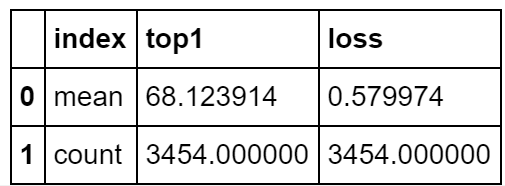
\includegraphics[width=0.7\linewidth]{final_acc_table.png}
\end{center}
   \caption{Test accuracy \& loss for the final model.}
\label{tab:acc}
\end{table}

\begin{table}[t]
\begin{center}
	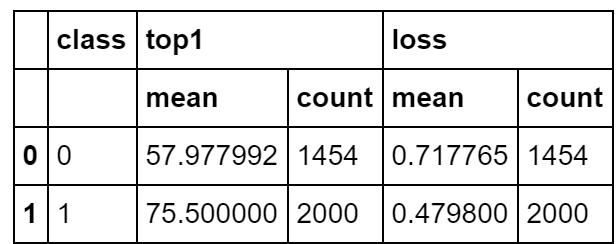
\includegraphics[width=0.7\linewidth]{final_acc_by_label_table.png}
\end{center}
   \caption{Test accuracy \& loss for each class label in the final model.}
\label{tab:acc2}
\end{table}

To evaluate these results, we compare our accuracy with a human benchmark. We recruited 17 UMass student participants to label 1,313 images with a total accuracy of 59.5\%, meaning that our classifier outperformed our human benchmark by 8.6\%.

Upon reviewing images, we suspect that this low human-accuracy is due to the fact that images of bike-designated roads do not always contain clear bike-designated infrastructure. For example, shared-lane arrows are clear indications of a bike-designated road, but are not present in every street-view image of bike-designated roads due to the positioning of the camera. On the other hand, our neural network predicted bike-designation based on scene attributes such as lighting, spatial envelope, textures, and objects, and did not rely exclusively on attributes such as shared-lane arrows or other infrastructure. In the following section, we explore qualitative results to better understand how our classifier determined relevant attributes for classification.

\subsection{Qualitative Results}
\label{sec:qualitative}
We generate class activation maps at the global average pooling layer of the ResNet model to visualize the parts of an image relevant to scene classification. Visualizing these results, we noticed that our neural network typically ignores the sky, as expected, and is highly activated on recognizable objects such as cars and light posts, as well as lane markings.

In addition, we examined the SUN scene attributes that were found in each image by adding a separate classification head branching from the ResNet global average pooling layer. Using the pre-trained final layer of the SUN attributes ResNet model, we could visualize what attributes were recognized by the convolutional layers in our model, which would be fed into our custom layers for bike-designation classification. Figures \ref{fig:bf_examples} and \ref{fig:nbf_examples} present example qualitative results for bike-designated and non-bike-designated street-view images respectively.

The results of the attributes demonstrate how fine-grained of a classification task the neural network faced. Both bike-designated and non-bike-designated roads contain similar attributes, given that all of the images are of outdoor, open roads, typically in suburban or rural settings. For example, ``man-made'', ``natural'', ``light'', and ``open-area'' are top attributes for images of both classes. While the distribution and order of top attributes changes from image to image, many attributes are shared between almost all images.

\begin{figure}[t]
\begin{center}
	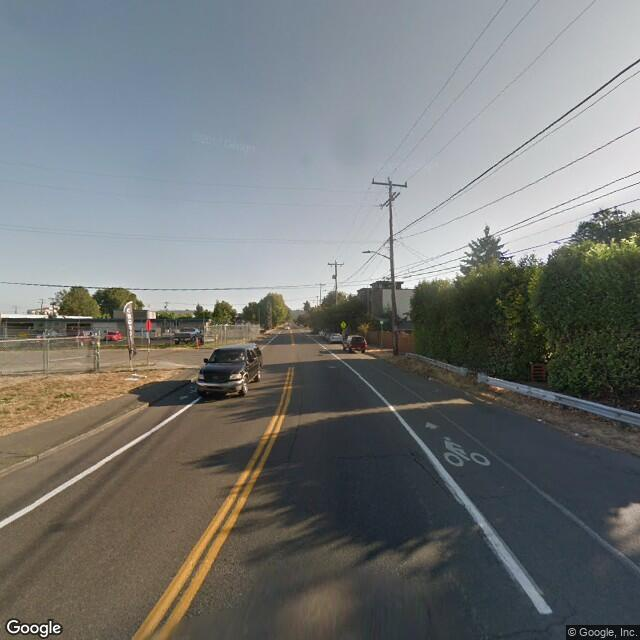
\includegraphics[width=0.32\linewidth]{bf.jpg} 
	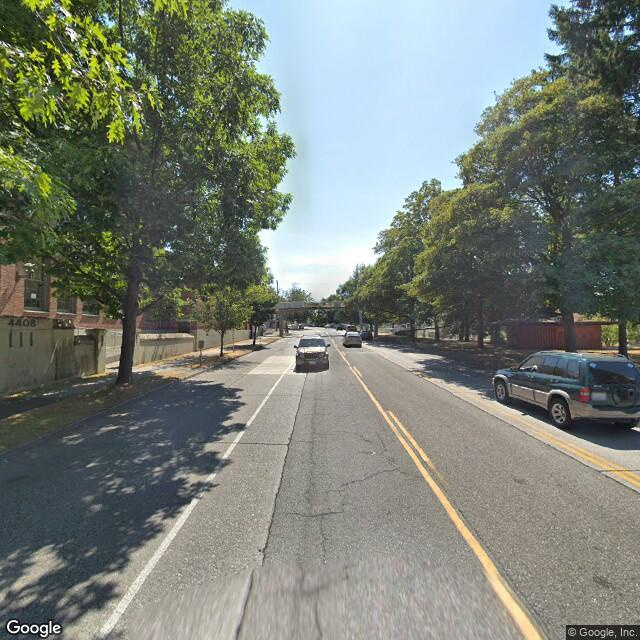
\includegraphics[width=0.32\linewidth]{bf_2.jpg} 
	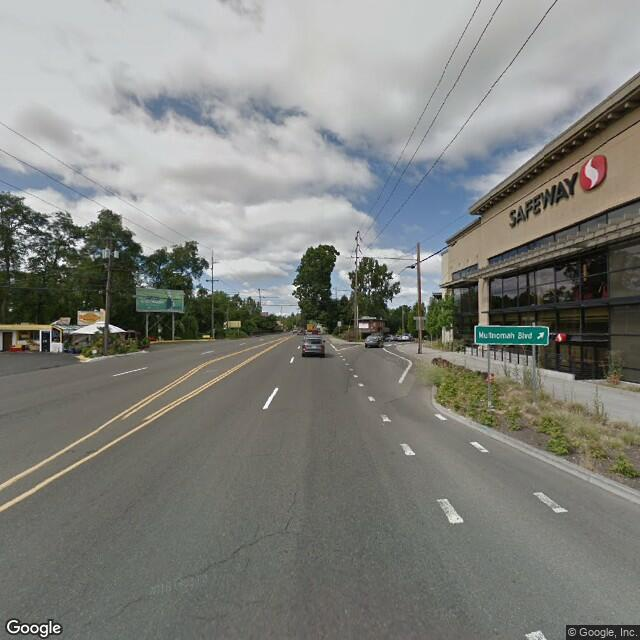
\includegraphics[width=0.32\linewidth]{bf_3.jpg} 	
	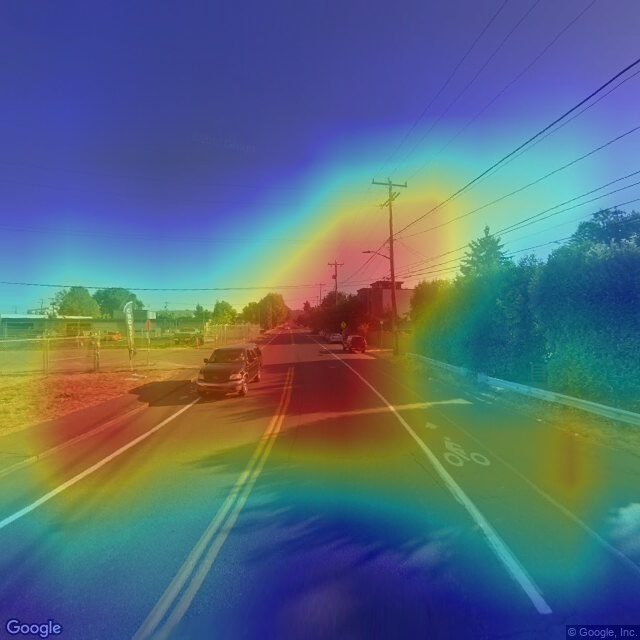
\includegraphics[width=0.32\linewidth]{bf_cam.jpg} 
	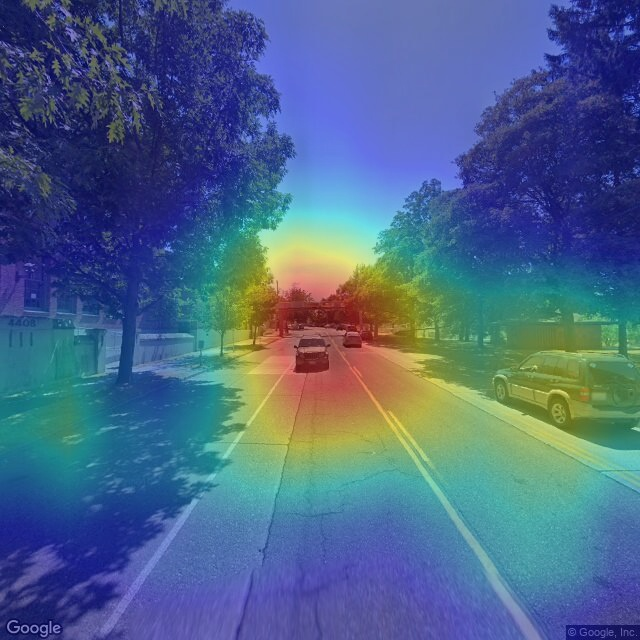
\includegraphics[width=0.32\linewidth]{bf_2_cam.jpg} 
	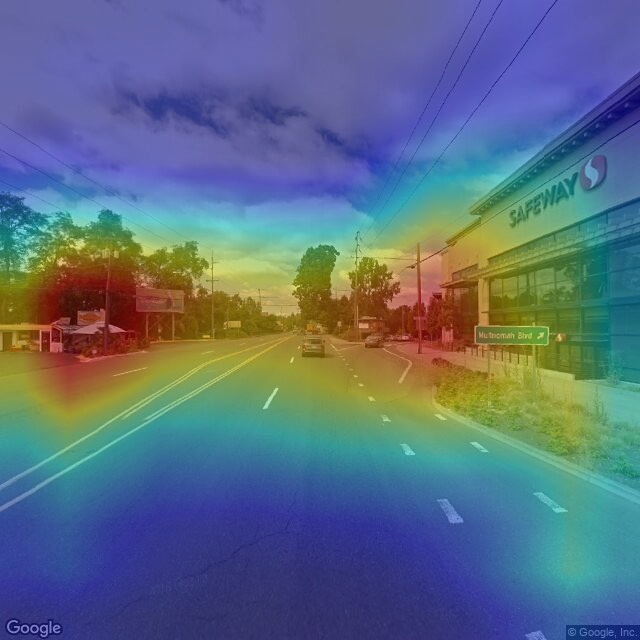
\includegraphics[width=0.32\linewidth]{bf_3_cam.jpg} 	
	
\vspace{-0.5cm}
\begin{multicols}{3}
\begin{framed}
open area \\
natural light \\
man-made \\
asphalt \\
driving  \\
biking  \\
far-away\\
 horizon \\
  transporting
\end{framed}
\begin{framed}

natural light\\
open area\\
driving\\
trees\\
man-made\\
asphalt\\
biking\\
foliage\\
leaves
\end{framed}
\begin{framed}
man-made\\
natural light\\
open area\\
driving\\
asphalt\\
biking\\
transporting\\
clouds\\
pavement
\end{framed}
\end{multicols}
\end{center}
   \vspace{-0.5cm}
   \caption{Bike-designated roads with class activation maps and top predicted attributes.}
\label{fig:bf_examples}
\end{figure}



\begin{figure}[t]
\begin{center}
	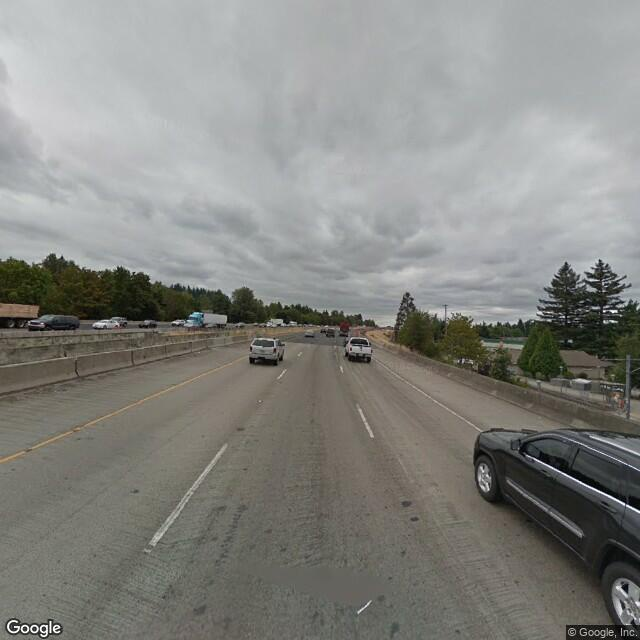
\includegraphics[width=0.32\linewidth]{non_bf.jpg} 
	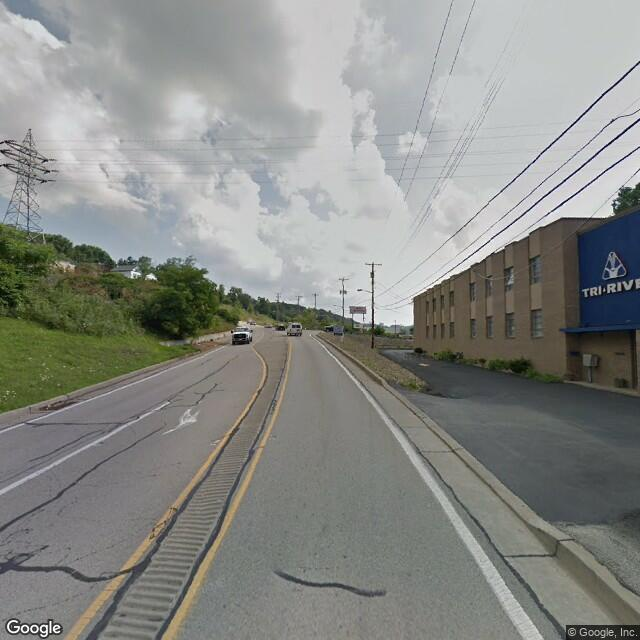
\includegraphics[width=0.32\linewidth]{non_bf_2.jpg} 
	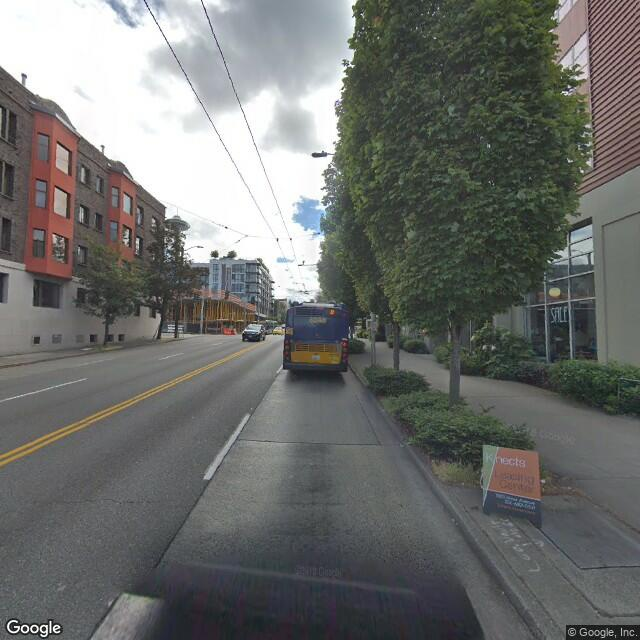
\includegraphics[width=0.32\linewidth]{non_bf_3.jpg} 	
	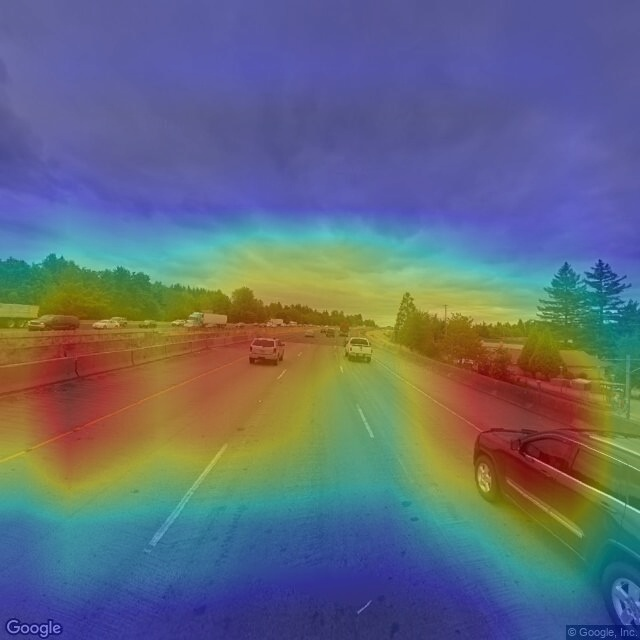
\includegraphics[width=0.32\linewidth]{non_bf_cam.jpg} 
	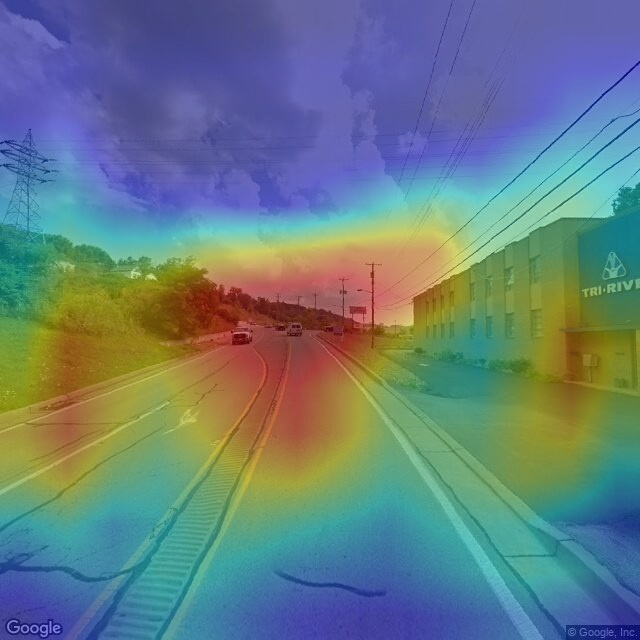
\includegraphics[width=0.32\linewidth]{non_bf_2_cam.jpg} 
	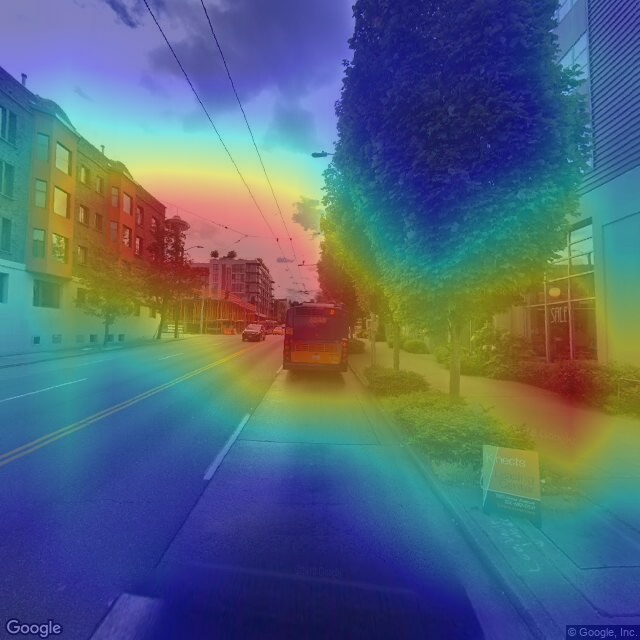
\includegraphics[width=0.32\linewidth]{non_bf_cam_3.jpg} 		
\vspace{-0.5cm}
\begin{multicols}{3}
\begin{framed}
open area\\
natural light\\
man-made\\
far-away horizon\\
driving\\
clouds\\
asphalt\\
transporting
\end{framed}
\begin{framed}

natural light\\
open area\\
man-made\\
driving\\
asphalt\\
biking\\
clouds\\
transporting\\
pavement

\end{framed}
\begin{framed}
man-made\\
natural light\\
open area\\
driving\\
asphalt\\
biking\\
pavement\\
transporting\\
no horizon
\end{framed}
\end{multicols}

\end{center}
   \vspace{-0.5cm}
   \caption{Bike-designated roads with class activation maps and top predicted attributes.}
\label{fig:nbf_examples}
\end{figure}




%%%%%%%%% CONCLUSION
\section{Conclusion}
\label{sec:conclusion}

\subsection{Findings}

We consider this project a successful, albeit initial, first undertaking to attempt to classify roads as bike-designated or not. By achieving greater than 50\% accuracy for both classes, and by even surpassing a human benchmark, we have demonstrated that neural networks are capable of learning to classify bike-designation in street-view images. 

In comparison to other classification tasks, an overall accuracy of 68.1\% seems low, especially for a binary classifier. However, the human benchmark we establish demonstrates that the classification task is non-trivial and differences between images of each class can be subtle.  

Nevertheless, we believe the performance of the model can be improved. To understand why the model performed this way, it is important to consider the qualitative and quantitative results of the experiments. The quantitative results in Section \ref{sec:quantitative} show that model learns to classify images well, but not equivalently for each class. The qualitative results in Section \ref{sec:qualitative} show that the class activation maps and the attributes produced by images of each class have cross-over. 

\subsection{Future Ideas}
This paper is a first attempt to classify whether images of roads are bike-designated or not. With additional funds, we could expand our dataset to include street-view images from additional cities, countries, and more rural areas; in addition, we could consider gathering multiple images per road, and even multiple images per point (for example, looking in both directions, or looking towards the sides of roads). Improving data quality is also important; for example, comparing the timestamps of road classification tags with Google Street View images to ensure data or labels are not outdated. Ensuring that all images are correctly labelled should also increase the performance of the model. We would also consider using additional sources of data, such as car dashboard cameras.

Another approach to improving this model would be changing our source of road classifications. Rather than classifying OpenStreetMap's bike-designation, the classifier could be fine-tuned to predict bike-friendliness (given rankings by cyclists) or bike-popularity (using cyclist GPS data similar to Strava Heatmap \cite{strava}). 


\nocite{patterson2014sun, DBLP:journals/corr/ZhouKLOT14, rundle2011using,Wang15l, DBLP:journals/corr/ZagoruykoK16,koehrsen2018blog}

{\small
\bibliographystyle{ieee}
\bibliography{cs682_final_report.bib}
}

\end{document}
